\chapter{Methods}

	\section{Experimental Animals}
		All experimental procedures were approved by the Florey Institute Animal Ethics committee and were conducted in accordance with the guidelines from the Animal Welfare Act 1992, The Animal Welfare Regulations (Vic) 1993 and the National Health \& Medical Research Council’s (NHMRC) Australian Code of Practice for the Care and Use of Animals for Scientific Purposes (8th Edition, listed as EA28 in the NHMRC Publications Online Catalogue under ‘Animal Ethics’). This study looked at the responses to visual stimuli in macaques (Macaca nemestrina) and tree shrews (Tupaia glis). The macaques were transported from the macaque colony (Monash Animal Research Platform) to the Melbourne Brain Centre (MBC) the day before the experiment and housed overnight and experimented on from the following day onwards. The tree shrews were obtained from the tree shrew colony at the MBC funded by the ARC Centre of Excellence in Integrative Brain Function. Macaque experiments typically lasted for 5 days and Tree Shrew experiments for 2 days. Data for this thesis was collected from a total of 6 macaques and 16 tree shrews.
		
	\section{Surgery and Anaesthesia}
	
		In all animals, initial anaesthesia was induced using a mixture of Ketamine (KETAMIL, Parnell Lab, Australia) and Xylazine (ILIUM XYLAZIL-20, Troy Laboratories, Australia; See table 1 for dosage). Once the animals were anaesthetised, venous cannulation was performed to help administer drugs and fluids. Following this, a tracheostomy was performed to administer artificial ventilation and anaesthesia during the experiment. Once the venous cannulation and tracheostomy were completed, the animals were mounted on a stereotaxic table in Horsley-Clarke co-ordinates. Artificial ventilation was provided using a respiratory pump (Harvard Apparatus, Massachusetts, USA) and anaesthesia was maintained using a gaseous mixture containing nitrous oxide, oxygen, carbogen and isoflurane (see table 1 for dosage). Paralysis was established and maintained using Vecuronium (NORCURON, Organon Australia Pty Ltd) administered intravenously (see table 1 for dosage). The animal's body temperature was maintained between 36 and 37 degrees using a servo controlled heating blanket. Silver electrodes were inserted into the frontal cortex and needles were placed in the skin on either side of the rib-cage to monitor EEG and ECG during the experiment. The end-tidal CO2 (between 3.6 and 3.8\%), the airway pressure (<10 mm/Hg) and core body temperature were also monitored during the experiment at regular intervals. Dosages of the various drugs used for the procedures detailed above are presented in Table 1.
		
		Using a microdrill, craniotomy was performed over the location of the primary visual cortex (V1) in macaques, and V1 and/or superior colliculus in tree shrews (SC; see table 1 for Horsley-Clarke co-ordinates). A durotomy was performed to remove the duramater, which both allowed a clear view of cortical surface for optical imaging as well as preserved the tip of the electrodes during microelectrode recordings. 
		
		The eyes of the animal were kept covered during surgery to protect the optics of the eye. Following surgery, the pupils were dilated using atropine sulphate (ATROPT 1\%, Sigma Pharmaceutical Pty Ltd, Australia) and rigid gas permeable contact lenses, matched for the curvature of the eyes, were fitted to prevent corneal drying. In the macaques and earlier tree shrew experiments, the eyes were refracted using a hand held projectoscope and corrective lenses were placed in front of the eye during the experiment. In the macaques, an artificial pupil (diameter= 4mm) was also placed in front of the eye. In later tree shrew experiments (9 animals), refraction was also performed during the experiment by showing animals sine-wave gratings of increasing spatial frequencies. The power of the lens where the spatial frequency resolution was the highest, was deemed the appropriate power. In most cases, the appropriate power was close to, if not the same as when no corrective lenses were added. As a result, corrective lenses were not used when they were not required, in order to limit any optical distortions the lenses may cause.
		
		Once recordings were completed, the experiment was terminated by administering the animal a lethal dose of pentobarbital sodium (200-300 mg, Merial Australia Pty Ltd) intravenously. The animals were then perfused intracardially using phosphate buffer solution (PB; 0.1M), the brain was fixed using a paraformaldehyde solution (PFA; 4\% Paraformaldehyde in 0.1M PB). The brain was removed and stored in a solution of 25\% sucrose (0.1M PB) for cryoprotection. The brain was later processed for histology.
		
		% insert table here
		
	\section{Electrophysiological Recordings}
	
		Single and multi-microelectrode recordings were made from the primary visual cortex (V1) and the superior colliculus of the tree shrews, and the macaque primary visual cortex as follows.
		
		\subsection{Single Electrode Recordings}
		
		A chamber was built around the opening using dental cement. Tungsten micro-electrodes (between 4 and 18 MΩ; FHC, Inc., ME, USA) were inserted into the cortex and the well was filled with with Agar solution (2\% Agar in 0.9\% Saline) for stability of recordings and protecting the cortex. The signal obtained from the microelectrode was first amplified (x 10,000 times; A-M Systems, WA, USA). An anti-aliasing filter (5000 Hz; A-M Systems) was applied to the signal and a HumBug noise eliminator (A-M Systems) was used to reduce 50 Hz line noise. Usually, this ‘raw signal’ was further filtered between 300 and 3000 Hz and the signal was digitised at 22.5 kHz using an analog to digital converter (Cambridge Electronic Design Limited, Cambridge, UK).  In some cases, the raw signal was also digitised in a separate channel for further analysis. The signal was also fed through an audio speaker and receptive field locations of the neurons were first plotted using the auditory feedback. The data was recorded and a template of the spikes was built using the Spike 2 software (CED, Cambridge, UK). Post stimulus time histograms (PSTHs) were built from the templated spikes for online analysis and the original signal was also saved for further analysis. At the end of each microelectrode track, electrolytic lesions were made by passing 6 μA of current for 6 to 7 seconds to identify the locations of the recordings.
		
		\subsection{Multielectrode Recordings}
		
		A 16 channel multi-electrode array (individual electrodes spaced 100 microns apart; Neuronexus Technologies, Ann Arbor, USA) was used to record from the macaque V1. The array was connected to a pre-amplifier (RA16PA, Tucker-Davis Technologies, USA), via a headstage (RA16CH), where the signal was amplified (x 10,000) and filtered (2.2 Hz to 7.5 kHz) and digitized at 12.5 kHz using TDT’s OpenEx software suite. Further digital filters were applied to separate the signal into an LFP stream (2.2-100 Hz) and a multi-unit stream (300-3000 Hz). These were saved for further analysis.
		
	\section{Stimuli}
	
	Stimuli were presented on a BARCO monitor (Frame rate= 80 Hz; Reference Calibrator Plus; Barco Video and Communications, Belgium). All stimuli were generated using the stimulus description language (SDL) and presented using the ViSaGe stimulus generator (VSG; Visage, Cambridge Research Systems, UK). To assess the stimulus preferred orientation of a unit, moving bars of 9 different orientations (18 directions) were presented to the neuron. The eye that gave the weaker or no response was occluded. Width of the bar was usually set as the narrowest bar that could still elicit a good response. The length, polarity, contrast and speed of the moving bar were all customized to elicit the best response from the neuron. Once the orientation of the stimulus was determined, the animal was presented with sine-wave gratings to determine the spatial frequency tuning of the neuron. To obtain the spatial frequency tuning, the contrast and size of the gratings were optimised and the spatial frequency was varied in steps of 0.1 and 0.3 cycles/$^o$. This was repeated at four different orientations 45$^o$ apart.
	
	\section{Data Analysis}
	
	All single unit and multi-unit recordings were templated using the Spike 2 software to isolate neurons. Each neuron at the recording site usually has a distinct set of spike parameters (shape, duration and amplitude of the components) and the spikes that were similar (with at least 60\% overlap) were grouped together as spikes from the same neuron. For each stimulus condition, a stimulus marker was produced and exported to the spike 2 software. The spikes from a neuron and the stimulus markers for each stimulus presentation were exported to a text file and analysed using custom software in MATLAB (The Mathworks Inc, MA, USA).
	
	The spikes that followed the same stimulus were gathered and displayed in a post stimulus time histogram (PSTH) so that each PSTH displays the response of the neuron to one stimulus (eg: the response to a bar of a certain orientation). In order to build a PSTH, the spikes were grouped in 20 ms intervals and the number of spikes in each bin was divided by the bin width (in seconds) to get the firing rate of the neurons (in spikes per second or Hz). The PSTH was then convolved with a Gaussian kernel (σ = 3 bins) to get the stimulus density function (SDF, see Figure 1 for example) to account for the variation in the trial-by-trial firing rate. Further measurements were performed on the SDF to define the response of the neurons to various stimuli.
	
	The response of the neuron to bars and gratings were quantified in different ways. For a moving bar, neurons showed a peak response when the bar passed over their receptive fields. Figure \ref{fig:mb} is the SDF of a neuron to a moving bar. As the bar moves over the receptive field, a peak is observed in the SDF (one for each direction). The response of the neuron is then the maximum response at each of the peaks (shown by the red circles).
		\begin{figure}[H]
		
		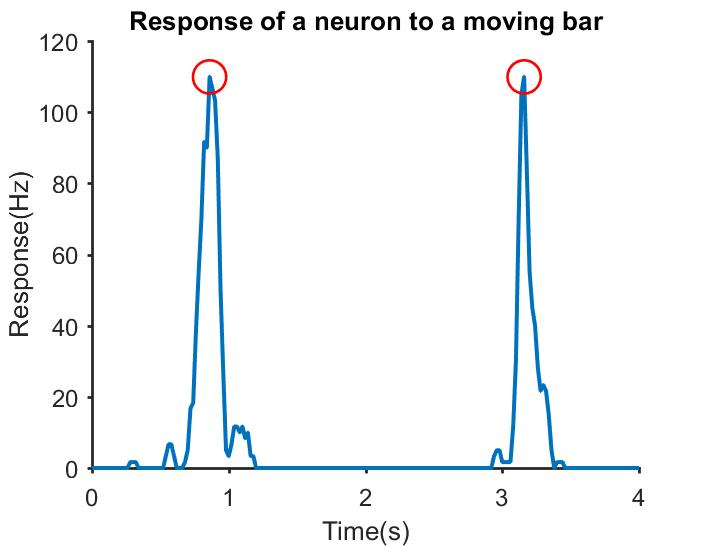
\includegraphics[width=\linewidth]{methods/SDF_movingbar.jpg}
		\caption{The SDF of a neuron’s response to a vertical bar moving bidirectionally. The maximum response in each direction is highlighted with red circles}
		\label{fig:mb}
		\end{figure}

	When shown gratings, neurons respond differently. A neuron, based on whether it demonstrates linear summation over its receptive field or not, responds differently to a grating. For example, ‘linear’ cells give a response modulated to the temporal frequency of a grating (see Figure \ref{fig:fourier}a; TF= 4Hz). A Fast Fourier Transform of the SDF is taken (Figure \ref{fig:fourier}b) and the peaks observed indicate that the respective frequencies have a high magnitude in the original signal. In this case, the FFT has two distinct peaks (red circles), the first one is at 0 Hz and the second one at 4Hz. The peak at 0 Hz is the F0 component of the response and is equal to the average of the signal in figure \ref{fig:fourier}a. The second peak is the F1 component and gives the fundamental frequency of the neuron’s modulated response (4 Hz). ‘Non-linear’ cells don’t show a modulated response to gratings, especially for higher spatial frequency gratings and as a result, the only distinct peak in the FFT corresponds to the F0 component (0 Hz). 
			\begin{figure}[H]
			
			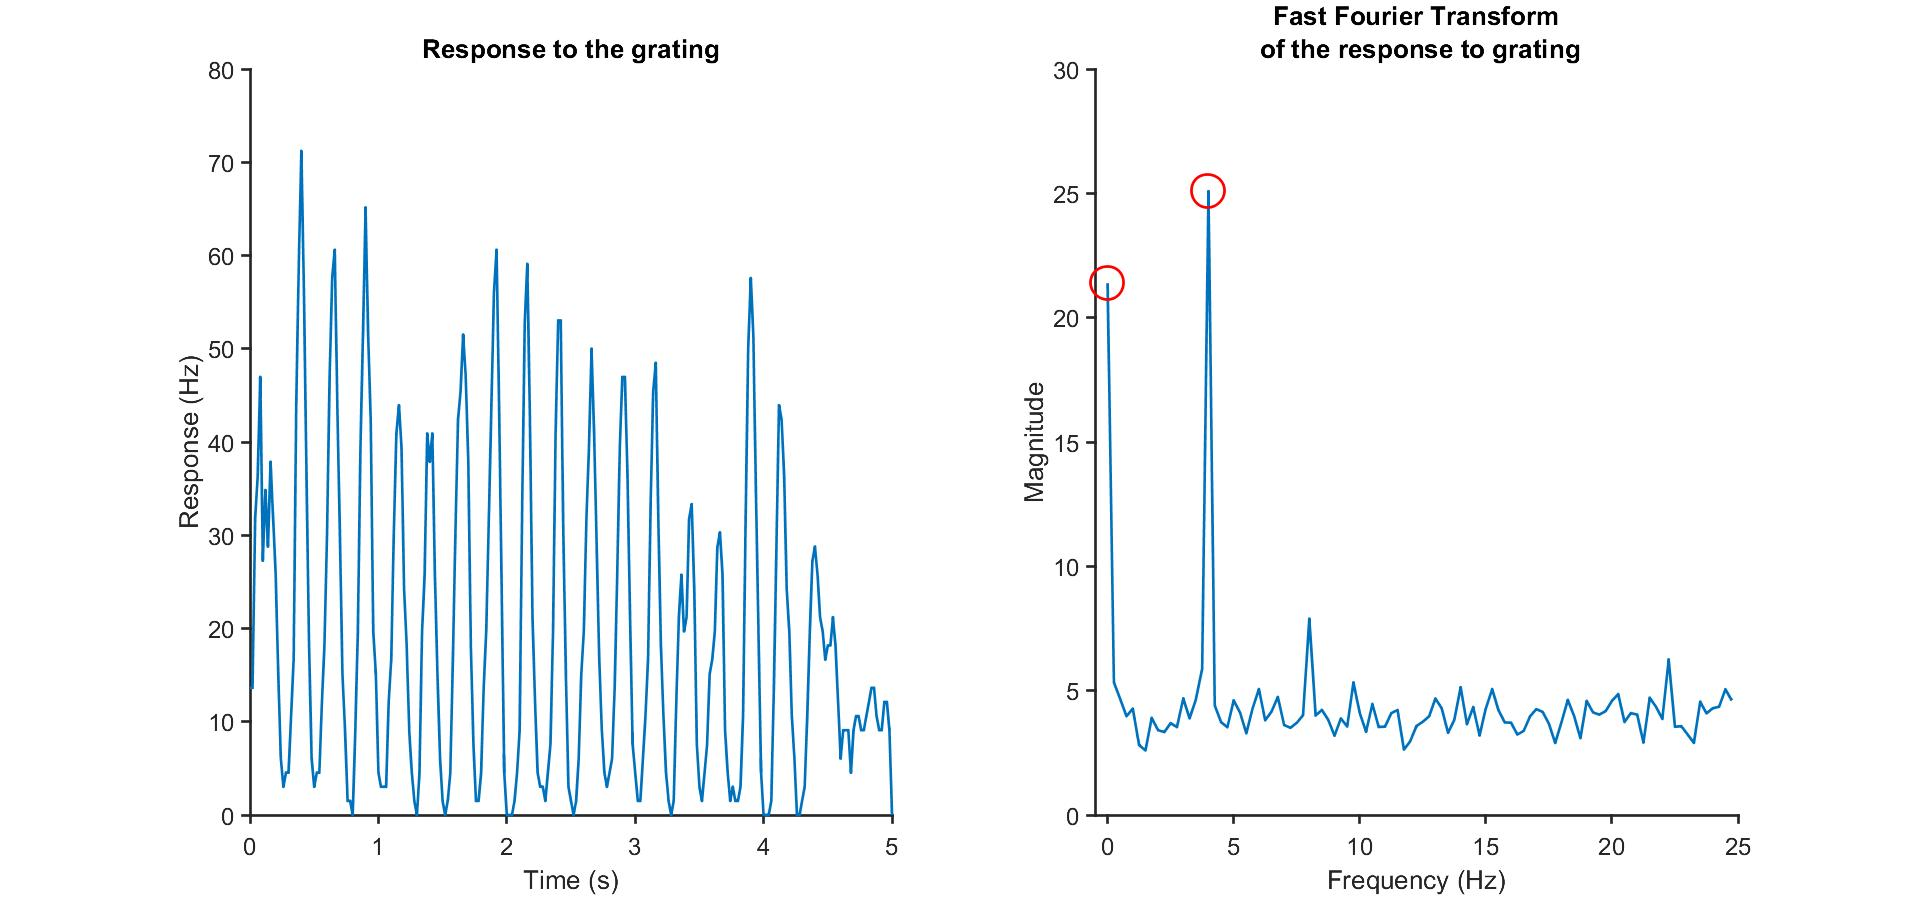
\includegraphics[width=\linewidth]{methods/Fourier.jpg}
			\caption{a) the SDF of a ‘linear’ cell. The first 4.3s was the stimulus presentation duration. A blank screen was presented for the last 0.7s. b) The fast fourier transform (FFT) of the signal in fig\ref{fig:fourier}a. There is a peak at the F0 component as well as at 4 Hz, which was also the temporal frequency of the sine wave grating.}
			\label{fig:fourier}
			\end{figure}
	
	Cells were first classified as linear or non-linear neurons – with our cortical and collicular data, comparable to the classical categories of simple and complex in the primary visual cortex (Hubel and Wiesel , 1962) and X and Y like in the lateral geniculate nucleus (Enroth-Cugell and Robson, 1966). This was done by taking the modulation index (Skottun et al., 1991) which is the ratio of the F0 and F1 components of the response. Traditionally, the modulation index is calculated by dividing the F1 component of the response by the F0 component. Neurons with modulation index less than 1 were classified as non-linear cells and cells with modulation index greater than 1.5 were classified as linear cells. Recently, a modified measure of the modulation index was proposed to measure linearity in the tree shrew primary visual cortex (Van Hooser et al., 2013). Using this measure, the range of values the modulation index could take was between 0 and 2 where neurons with modulation index less than 1 were classified as non-linear cells and where neurons with modulation ratio between 1 and 2 were classified as linear cells. This measure of modulation index was chosen to enable comparison with earlier tree shrew studies. For non-linear cells, the F0 component of the response was used for further analysis while for linear cells, the F1 component was used. From the response of the neuron to drifting sinusoidal gratings of increasing spatial frequencies, the spatial frequency tuning curves of the neuron was constructed and the peak spatial frequency and the half width at half height were calculated.
	
	\section{Histology}
	
	After the experiment, the tissue was processed for histology as follows. The brain was stored in a 25\% sucrose solution until it sank. This was to ensure that the tissue was cryoprotected. The brain was cut into blocks so that only the areas of interest were sectioned. The brain was frozen and 50 micron sections were made using a cryostat (Leica CM3050S, Leica Microsystems, Nussloch, Germany). The sections were collected and stored in a Sodium Azide solution (0.1\% in 0.1M PB) till they could be mounted on gelatinised slides after which they were dried overnight and stained.
	
	\subsection{Cresyl violet staining}
	
	First the sections were dehydrated using increasing concentrations of ethanol solution. Then, chloroform was used to de-fatten the sections. This was followed by rehydrating sections in decreasing concentrations of ethanol. The sections were then stained using Cresyl Violet Acetate solution (0.1\%, Sigma-Aldrich, Inc., USA) and differentiated using a solution of 5\% percent acetic acid in 95\% ethanol. The sections were then fixed in histolene and the slides were coverslipped.
	
	\subsection{Track Reconstruction}
	
	In order to reconstruct electrode tracks, the electrolytic lesions were located under a light microscope and digitised (Zeiss Axiocam Digital Camera, Zeiss, Germany). The shrinkage was calculated by comparing the recorded and observed distances between lesions using Adobe Illustrator(Adobe systems software Ltd). The shrinkage calculation was used to accurately determine the actual depth of the units recorded. In tree shrew V1, based on the location of the unit, it was classified as layer 4 or layer 2/3. In the shrew superior colliculus, the units were categorized as either belonging to the superficial or deeper layers of the superior colliculus.
	
	\section{Optical Imaging of Intrinsic Signals}
	
	Optical imaging of intrinsic signal is a high resolution imaging method that is used to detect the changes in blood oxygenation level in areas of neuronal activity. As a result of neuronal activity there is increased oxygen consumption in the surrounding tissue which leads to an increase in the level of de-oxy haemoglobin in the blood. This leads to a difference in reflectance in the tissue between regions where there is oxygenated and de-oxygenated blood and it is this signal that OI detects. This is the same signal as the fMRI BOLD signal but optical imaging has one key advantage over BOLD imaging. Whereas the fMRI signal has the resolution in the scale of millimetres, OI can detect  signals at at least one order of magnitude higher resolution, allowing us to visualize the organization of neuronal activity at the scale of cortical columns. So, Optical imaging was used to image the functional activity of the macaque primary visual cortex. 
	\subsection{The apparatus}
	
	In order to acquire OI maps of the primary visual cortex, first, a tandem lens macroscope was attached to a slow-scanning CCD camera. A light source is used to provide illumination for the duration of the imaging and the acquired frames were converted into a digital signal using an analog to digital converter. The specifications of these equipments are detailed below.
	
	\subsubsection{Macroscope and camera}
	
	A tandem lens macroscope was constructed by arranging two camera lenses (Pentax lenses, f= 50mm) end-to-end. This macroscope had a shallow depth of field which allowed us to focus at a specific depth below the surface of the cortex. In this manner, we acquired the blood flow changes related to the neuronal activity at the depth where the lens was focused. The macroscope was connected to a slow scan CCD camera (Teli CS 8310B; Ts’o et al., 1990) which acquired and transmitted images to the imaging system (VDAQ Imager 3001, Optical Imaging, Rochester, NY). 
	
	\subsubsection{The Chamber}
	
	As the images were acquired in-vivo in an anaesthetized macaque, there was the possibility of the image being contaminated by movement artefacts caused by the animal’s respiration and heartbeat. To reduce this, a metal chamber (diameter= 10 mm) was placed on the skull surrounding the exposed cortical area. It was sealed in place using dental cement (Dentimex VA, Netherlands) and ensured that no leaks were present. Once the chamber was fixed to the skull, it was filled with Silicone oil (Polydimethylsiloxane 200 fluid, viscosity 50 cSt, Sigma-Aldrich, Inc., USA) and sealed with a coverslip. In the macaque, due to the angle of the imaged area, we used a metal chamber without the metal pipes traditionally used to fill the chamber. The cylinder was overfilled with Silicone oil and the coverslip tightened. Where bubbles were present, the process was repeated until a clear view of the cortex was achieved.
	
	\subsubsection{The Illumination System}
	A circular fibre-optic attachment was connected to the camera lens for uniform illumination during optical imaging. First, a green light filter (545 nm) was used to obtain an image of the cortical surface with blood vessel landmarks (the green image). Then a longer wavelength (630 nm) filter was used for imaging. This wavelength of light was used because it was shown to reliably isolate the haemodynamic changes related to neuronal activity. Shorter wavelength lights (< 600 nm) reveal more of the blood volume changes while light of wavelength longer than 630 nm primarily detected light scatter effects. Light at 630 nm was the longest wavelength of light we could use to ensure maximum penetration of the light into the cortex while still imaging the haemodynamic changes.
	
	\subsection{Image acquisition}
	
	\subsubsection{Stimulus presentation}
	
	Stimulus was generated by the ViSaGe system and displayed on the BARCO monitor as described below. The Visage and the camera were synchronized by the means of an optical imaging interface (VDAQ Imager 3001, Optical Imaging, Rochester, NY). The interface started the camera when the stimulus presentation began. The stimuli were eight full field, bidirectional, square wave gratings (contrast =100\%; Spatial Frequency = 1-2.5 cycles/degree; Temporal Frequency = 1.5 Hz) of changing orientations. The stimulus was presented for 7.2 seconds, followed by a 10 second blank. This inter-stimulus interval allowed the OI signal to return to baseline. This was repeated 50 times to improve the signal-to-noise ratio.
	
	\subsubsection{Image acquisition system}
	
	The macroscope was focused below the surface of the cortex between 550 and 700 μm. Then, when the stimulus was presented, the Imager 3001 simultaneously started the camera which acquired 18 frames, each 400 ms long while the stimulus was presented. There was no image acquisition during the inter stimulus blank time. In order to get an image of the cortex at rest, a blank stimulus was presented for 7.2 s, followed by a 10 s interstimulus interval. The camera had a 14-bit bit-depth, which allowed the detection of very small variations in the OI signal. The individual frames for each block (10 trials per block) were first saved by the imaging system and exported to MATLAB for further analysis.
	
	\subsection{Analysis of Intrinsic Signals}
	
	\subsubsection{Pre-processing of the data}
	
	Prior to the analysis, the data acquired had to be corrected for luminance artefacts. We did this by averaging frame numbers 3 to 16 from all the 50 trials for each stimulus condition (between 1200 and 6800 ms) and dividing it by the average of the first frame across 50 trials. These frames were chosen as the signal from OI when using the 630 nm light is biphasic (see figure \ref{fig:oit}). The initial signal first dips below the baseline and then increases later, peaking at approximately 5 s after the stimulus was presented. This is generally consistent with the time-course of the de-oxyhaemoglobin concentration (Malonek and Grinvald, 1996). To account for the illumination effects, the first frame subtraction method was employed to create a differential map. In this method, the blank was taken as the first frame and the activity of all other frames are calculated as the difference of the frame from the ‘blank’ frame. This division by the blank is equivalent to subtracting and dividing by the blank since the optical imaging signal is relatively small (see Pouratian \& Toga, 2002).
	
		\begin{figure}[H]
		
		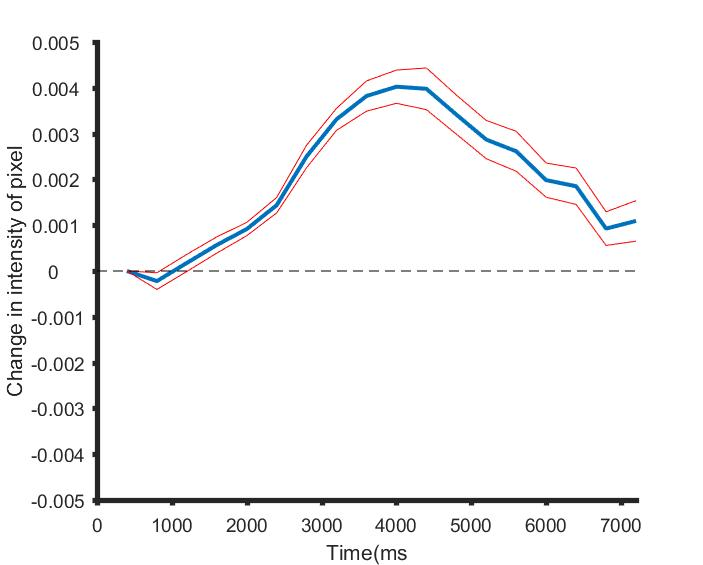
\includegraphics[width=\linewidth]{methods/OI_timecourse2.jpg}
		\caption{The time course of the OI haemodynamic signal for the duration of the stimulus presentation. The deoxyhaemoglobin levels briefly increase before decreasing, leading to a decrease in pixel intensity followed by an increase.}
		\label{fig:oit}
		\end{figure}
	
	\subsubsection{Obtaining single condition and orientation maps}
	
	The differential map is bandpass filtered in order to obtain the single condition map. This is done as follows. First the differential map is low pass filtered using a Gaussian kernel with a large sigma value (312.5 microns). The low pass filtered map is subtracted from the differential map to obtain the highpass filtered map which is once again filled with a Gaussian kernel with a small sigma value (100 microns). The resulting map is the single condition map (SCM; see figure 4).
	
	\begin{figure}[H]
		
		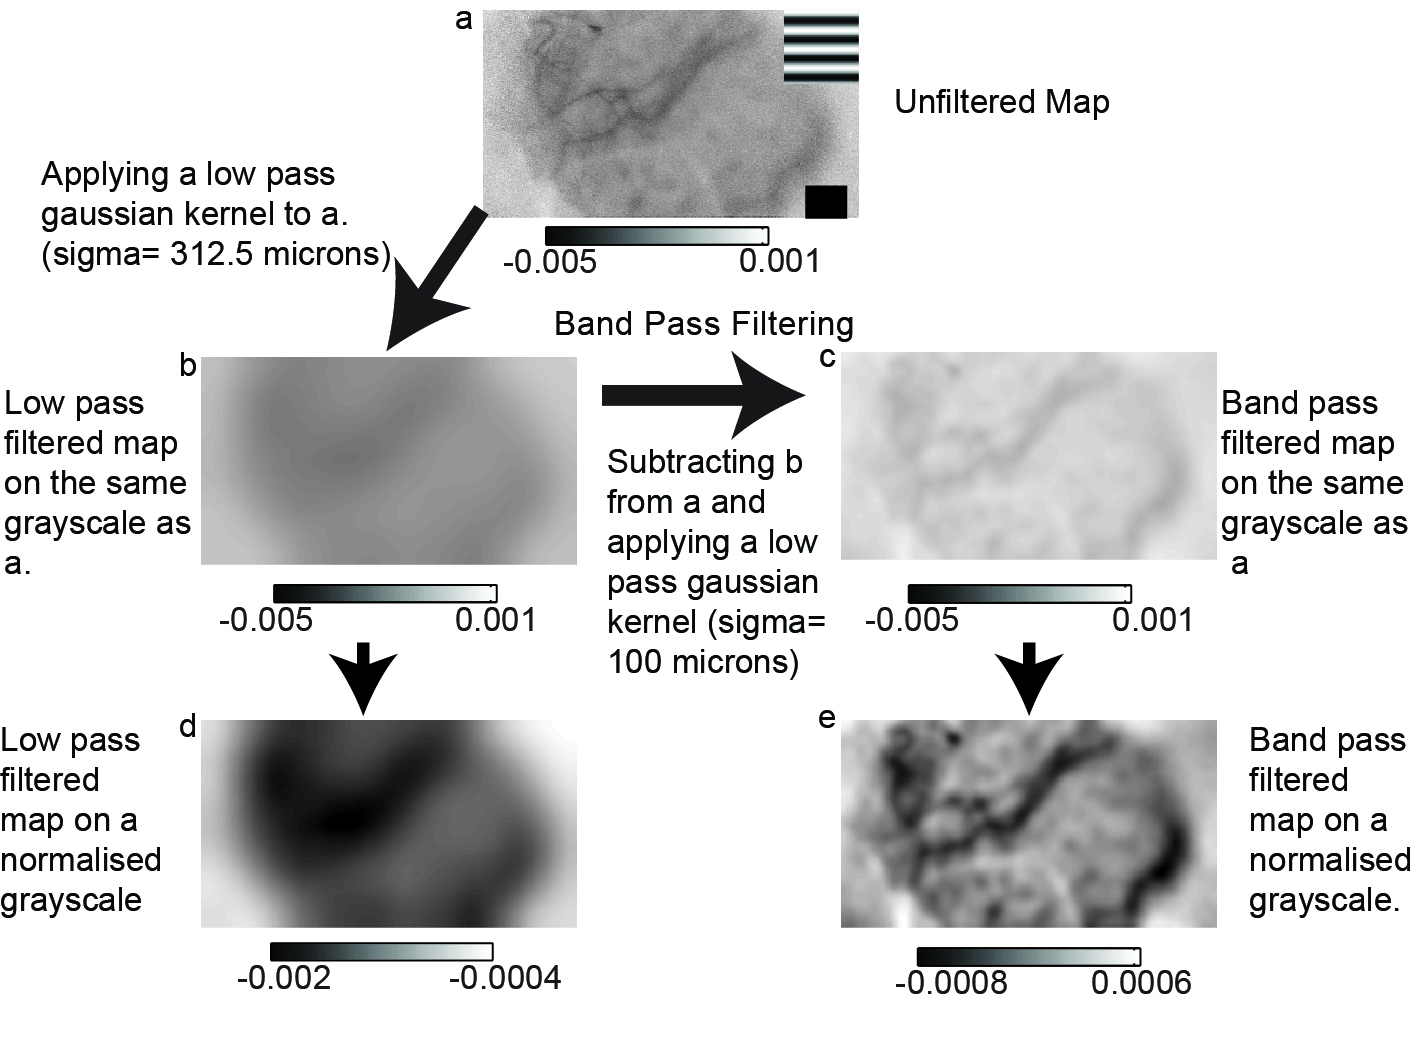
\includegraphics[width=\linewidth]{methods/filters.jpg}
		\caption{The filtering process used to generate single condition maps. The differential maps are first high-pass filtered to remove spatial scale signals and a smaller low-pass, smoothing filter was used to remove the high spatial noise.}
		\label{fig:filters}
	\end{figure}
	
	The single condition maps obtained for each orientation are then vector averaged (Swindale, 1998) to create the orientation domain map.